\section{4. Определения предела функции в точке по Коши и по Гейне, их равносильность. Свойства пределов функции. Предел композиции. Критерий Коши существования предела функции. Односторонние пределы функции, теорема об односторонних пределах монотонной функции.}

    Пусть $E \subset \R, \ a,b \in \overline{\R}, f: E \longrightarrow \R$
    
    \begin{definition}{\textit{Коши.}}
        Точка $b$ называется \textit{пределом} функции $f$ в точке $a$, если $a$ -- предельная точка множества $E$ и
        \[\forall \epsilon > 0 \ \exists \delta > 0 \ \forall x \in E \ (x \in \mathring{B_{\delta}}(a) \Rightarrow f(x) \in B_{\epsilon}(b))\]
        Пишут $\lim_{x \rightarrow a} f(x) =  b$, или $f(x) \rightarrow b$ при $x \rightarrow a$.
    \end{definition}
    
    \begin{center}
        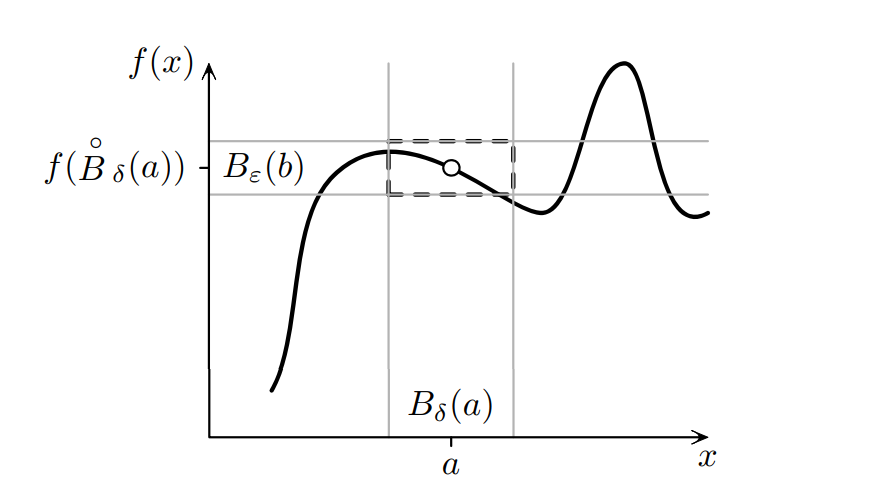
\includegraphics[width=0.5\textwidth]{colloq3.png}
    \end{center}
    
    \begin{definition}{\textit{Гейне.}}
        Точка $b$ называется \textit{пределом} функции $f$ в точке $a$, если $a$ -- предельная точка $E$ и выпонено следующее:
        \[\forall\{x_{n}\} \subset E \setminus \{a\} \ (x_{n} \rightarrow a \Rightarrow f(x_{n}) \rightarrow b )\]
        Пишут $\lim_{x \rightarrow a} f(x) =  b$, или $f(x) \rightarrow b$ при $x \rightarrow a$.
    \end{definition}
    
    \begin{theorem}
        Определения пределов по Коши и по Гейне равносильны.
    \end{theorem}

    \begin{proof}
        Пусть $f: E \longrightarrow R$, $a$ -- предельная точка множества $E$.
        \\
        $\Rightarrow$ Пусть $b = \lim_{x \rightarrow a} f(x)$ по Коши.
        Рассмотрим произвольную $\{x_{n}\} \subset E \setminus \{a\}$, $x_{n} \rightarrow a$. Докажем, что $f(x_{n}) \rightarrow b$.
        \\
        Зафиксируем $\epsilon > 0$. По определению предела $\exists \delta > 0 \ \forall x \in E \ (x \in \mathring{B_{\delta}}(a) \Rightarrow f(x) \in \overset{}{B_{\epsilon}}(b))$. Т.к. $x_{n} \rightarrow a$, то $\exists N \in \N \ \forall n \geq N \ (x_{n} \in \overset{}{B_{\delta}}(a))$. По условию $x_{n} \in E \setminus \{a\}$ и, значит, $\forall n \geq N \ (x_{n} \in \mathring{B_{\delta}}(a) \cap E)$. Тогда $\forall n \geq N: f(x_{n}) \in \overset{}{B_{\epsilon}}(b) \Rightarrow f(x_{n}) \rightarrow b$. Определение предела по Гейне выполняется. 
        \\
        $\Leftarrow$ Пусть $b$ -- предел $f$ в точке $a$ по Гейне. Покажем, что $b$ -- предел функции по Коши. Пусть так, и предположим, что $b$ не является пределом $f$ в точке $a$ по Коши. Тогда 
        \[\exists \epsilon > 0 \ \forall \delta > 0 \ \exists x \in E (x \in \mathring{B_{\delta}}(a) \text{ и } f(x) \notin \overset{}{B_{\epsilon}}(b))\]
        Положим $\delta = \frac{1}{n}$, $n \in \N$ и соответствующее значение x обозначим $x_{n}$. По построению $\{x_{n}\} \subset E \setminus \{a\}$ и $x_{n} \rightarrow a$ (т.к. $x_{n} \in \mathring{B_{\frac{1}{n}}}(a)$). По определению предела по Гейне $f(x_{n}) \rightarrow b$, значит $\exists N \in \N \ \forall n \geq N \ (f(x_{n}) \in \overset{}{B_{\epsilon}}(b))$. Противоречие по построению (все $f(x_{n}) \notin \overset{}{B_{\epsilon}}(b)$).
    \end{proof}

    Пусть $f,g,h: E \longrightarrow \R$, $a$ -- предельная точка множества $E$.

    \begin{definition}
        $f: X \longrightarrow Y$, $A \subset X$. \textit{Сужением} $f$ на множестве $A$ называется
        \[f|_{A}: A \longrightarrow Y, (f|_{A})(x) = f(x) \ \forall x \in A\]
    \end{definition}
    
    \begin{enumerate}
        \item (о единственности) Если $\lim_{x \rightarrow a} f(x) = b$ и $\lim_{x \rightarrow a} f(x) = c$, то $b = c$
        \begin{proof}
            Рассмотрим произвольную $\{x_{n}\} \subset E \setminus \{a\}$, $x_{n} \rightarrow a$. По определению Гейне:
            \[f(x_{n}) \rightarrow b \text{ и } f(x_{n}) \rightarrow c\]
            В силу единственности предела последовательности $b = c$.
        \end{proof}
        \item (о пределе по подмножеству) Если $\lim_{x \rightarrow a} f(x) = b$ и $a$ -- предельная точка множества $D \subset E$, то $\lim_{x \rightarrow a} f|_{D}(x) = b$.
        \begin{proof}
            Рассмотрим $\{x_{n}\} \subset D \setminus \{a\}$, $x_{n} \rightarrow a$. Тогда
            \[f|_{D}(x_{n}) = f(x_{n}) \rightarrow b\]
            По определению Гейне, $b = \lim_{x \rightarrow a} f|_{D}(x)$.
        \end{proof}
        \item (о зажатой функции) Пусть $\exists \sigma > 0 \ \forall x \in \overset{o}{B_{\sigma}} (a) \cap E \ (f(x) \leq h(x) \leq g(x))$. Пусть $\lim_{x \rightarrow a} f(x) = b$, $\lim_{x \rightarrow a} g(x) = b$. Тогда $\exists \lim_{x \rightarrow a} h(x) = b$.
        \begin{proof}
            Рассмотрим $x_{n} \subset E \setminus \{a\}$, $x_{n} \rightarrow a$. Тогда $\exists n_{0} \ \forall n \geq n_{0} (x_{n} \in \overset{o}{B_{\sigma}}(a) \cap E)$ и, значит, $f(x_{n}) \leq h(x_{n}) \leq g(x_{n})$. По условию $f(x_{n}) \rightarrow b$, $g(x_{n}) \rightarrow b$. Тогда, по свойству предела последовательности, $h(x_{n}) \rightarrow b \Rightarrow b = \lim_{x \rightarrow a} h(x)$.
        \end{proof}
        \item (арифметические операции с пределами) Пусть $\lim_{x \rightarrow a} f(x) = b$, $\lim_{x \rightarrow a} g(x) = c$. Тогда справедливы следующие утверждения:
        \\
        1. $\lim_{x \rightarrow a} (f(x) \pm g(x)) = b \pm c$.
        \\
        2. $\lim_{x \rightarrow a} (f(x) \cdot g(x)) = b \cdot c$.
        \\
        3. Если $c \neq 0$ и $g(x) \neq 0 \ \forall x \in E$, то $\lim_{x \rightarrow a} (\frac{f(x)}{g(x)}) = \frac{b}{c}$.
        
        Заключение следует понимать так: если существует величина справа, то существует величина слева и они равны.
        \begin{proof}
            Рассмотрим произвольную последовательность $\{x_{n}\} \in E$ с условиями $x_{n} \to a$ и $x_{n} \neq a$. Тогда $f(x_{n}) \to b$ и $g(x_{n}) \to c$. По свойствам предела последовательности $f(x_{n}) \pm g(x_{n}) \to b \pm c$, $f(x_{n}) \cdot g(x_{n}) \to b \cdot c$, $\frac{f(x_{n})}{g(x_{n})} \to \frac{b}{c}$. Осталось воспользоваться определением предела по Гейне.
        \end{proof}
        \item (о локализации) Если $\exists \sigma > 0 \ \forall x \in \overset{o}{B_{\sigma}}(a) \cap E \ (f(x) = g(x))$ и $\lim_{x \rightarrow a} f(x) = b$, то $\exists \lim_{x \rightarrow a} g(x) = b$.
        \begin{proof}
            Если в определении Коши предел $f$ для $\epsilon > 0$ подходит $\delta > 0$, то в поределении Коши предел $g$ подходит $\delta' = min\{\delta, \sigma\}$.
        \end{proof}
        \item (о локализации ограниченности) Если $\exists \lim_{x \rightarrow a} f(x) \in \R$, то $\exists C > 0 \ \exists \delta > 0 \ \forall x \in \overset{o}{B_{\delta}}(a) \cap E \ (|f(x)| \leq C)$.
        \begin{proof}
            Пусть $\lim_{x \rightarrow a} f(x) = b$. Тогда $\exists \delta > 0 \ \forall x \in \overset{o}{B_{\delta}}(a) \cap E \ (b - 1 < f(x) < b + 1)$. Положим $c = |b| + 1$. Тогда $|f(x)| < c$.
        \end{proof}
        \item (О пределе композиции.) Пусть $E, D \subset \R$ и $f: E \longrightarrow D$ и $g: D \longrightarrow \R$, такие что $\lim_{x \rightarrow a} f(x) = b$ и $\lim_{y \rightarrow b} g(y) = c$. Пусть выполнено одно из двух условий: 
        \\
        1) $f(x) \neq b$ в некоторой проколотой окрестности множества $a$ или 
        \\
        2) $g(b) = c$. Тогда $\lim_{x \rightarrow a} g(f(x)) = c = \lim_{y \rightarrow b} g(y)$.
        \begin{proof}
            Зафиксируем $\epsilon > 0$. По определению предела
            \[\exists \sigma > 0 \ \forall y \in \overset{o}{B_{\sigma}}(b) \cap D \ (g(y) \in \overset{}{B_{\epsilon}}(c))\]
            \[\exists \delta > 0 \ \forall x \in \overset{o}{B_{\delta}}(a) \cap E \ (f(x) \in \overset{}{B_{\sigma}}(b))\]
            1) Уменьшая $\delta$, если необходимо, можно считать, что $f(x) \neq b$ на $\overset{o}{B_{\delta}}(a) \cap E$. Тогда $f(x) \in \overset{o}{B_{\sigma}}(b) \cap D$. Поэтому $g(f(x)) \in \overset{}{B_{\epsilon}}(c) \Rightarrow \lim_{x \rightarrow a} g(f(x)) = c$.
            \\
            2) Если $f(x) = b$ для некоторого $x \in \overset{o}{B_{\delta}}(a)$, то $g(f(x)) = c \in \overset{}{B_{\epsilon}}(c)$. Поэтому $\forall x \in \overset{o}{B_{\delta}}(a) \cap E \ (g(f(x)) \in \overset{}{B_{\epsilon}}(c)) \Rightarrow \lim_{x \rightarrow a} g(f(x)) = c$.
        \end{proof}
    \end{enumerate}

    \begin{theorem} Критерий Коши.\\
        Пусть $f : E \longrightarrow \R$, $a$ -- предельная точка множества $E$. Функция $f$ имеет конечный предел в точке $a$ тогда и только тогда, когда 
        \[\forall \epsilon > 0 \ \exists \delta > 0 \ \forall x, x' \in \mathring{B_{\delta}}(a) \cap E \ (|f(x) - f(x')| < \epsilon)\]
    \end{theorem}
    
    \begin{proof} \ \\
        $\Rightarrow$ Пусть $\lim_{x \to a} f(x) = b$. Зафиксируем $\epsilon > 0$. По определению предела функции $\exists \delta > 0 \ \forall x \in \mathring{B_{\delta}}(a) \cap E \ (|f(x) - b| < \frac{\epsilon}{2})$. Тогда $\forall x, x' \in \mathring{B_{\delta}}(a) \cap E$ имеем
        \[|f(x) - f(x')| \leq |f(x) - b| + |f(x') - b| < \frac{\epsilon}{2} + \frac{\epsilon}{2} = \epsilon\]
        Так как $\epsilon > 0$ -- любое, то условия теоремы выполняются.
        \\
        $\Leftarrow$ Пусть $f$ удовлетворяет условию теоремы. Зафиксируем $\epsilon > 0$ и подберем соответствующее \\ $\delta > 0$. Рассмотрим произвольную последовательность точек $x_{n} \in E$ со свойствами $x_{n} \to a$ и $x_{n} \neq a$. Найдется такой номер $N$, что $\forall n \geq N \ (x_{n} \in \mathring{B_{\delta}}(a) \cap E)$ и, значит, $\forall n, m \geq N \ (|f(x_{n}) - f(x_{m})| < \epsilon)$. Таким образом, последовательность $\{f(x_{n})\}$ -- фундаментальна. По критерию Коши для последовательностей $\{f(x_{n})\}$ сходится к некоторому числу $b$. Рассмотрим еще последовательность точек $y_{n} \in E$ со свойствами $y_{n} \to a$ и $y_{n} \neq a$. Тогда $\forall \epsilon > 0 \ \exists n_{0} \in \N \ \forall n \geq n_{0} \ (x_{n}, y_{n} \in \mathring{B_{\delta}}(a) \cap E)$ и, значит, по условию $\forall n \geq n_{0} \ (|f(x_{n}) - f(y_{n})| < \epsilon)$. Это означает, что $f(x_{n}) - f(y_{n}) \to 0$, так что $f(y_{n}) \to b$. По определению Гейне $b = \lim_{x \to a} f(x)$.
    \end{proof}

    \begin{definition}
        Если $a$ -- предельная точка $(a, +\infty) \cap E$, то предел сужения $f|_{(a, +\infty) \cap E}$ в точке $a$ называется \textit{пределом справа} функции $f$ в точке $a$ и обозначается $f(a+0)$, или $\lim_{x \to a+0} f(x)$.
        \\
        Если $a$ -- предельная точка $(-\infty, a) \cap E$, то предел сужения $f|_{(-\infty, a) \cap E}$ в точке $a$ называется \textit{пределом слева} функции $f$ в точке $a$ и обозначается $f(a-0)$, или $\lim_{x \to a-0} f(x)$.
        \\
        Пределы функции слева и справа называются \textit{односторонними}.
    \end{definition}
    
    \begin{definition}
        Пусть $f: E \longrightarrow \R$, и $D \subset E$.\\
        Функция $f$ называется \textit{нестрого возрастающей (нестрого убывающей)} на $D$, если для любых $x, x' \in D$ из условия $x < x'$ следует $f(x) \leq f(x') (f(x) \geq f(x'))$.\\
        Если вместо $\leq (\geq)$ написать < (>), то функцию называют \textit{строго возрастающей (строго убывающей)}.\\
        Нестрого возрастающие и нестрого убывающие функции называются \textit{монотонными}.
    \end{definition}
    
    \begin{theorem}{Об односторонних пределах монотонной функции}\\
        Пусть $a, b \in \overline{\R}$, $a < b$. Если функция $f$ нестрого возрастает на $(a, b)$, то существуют $\lim_{x \to b-0} f(x) = \sup_{x \in (a, b)} f(x)$ и $\lim_{x \to a+0} f(x) = \inf_{x \in (a, b)} f(x)$.\\
        В случае нестрогого убывания $\sup$ и $\inf$ меняются местами.\\
    \end{theorem}
    
    \begin{proof}
        Предположим, что $f$ нестрого возрастает на $(a, b)$. Пусть $s = \sup_{(a,b)} f(x)$. По определению супремума для любого $r < s$ существует такое $x_{r} \in (a,b)$, что $r < f(x_{r})$. Тогда в силу возрастания $r < f(x) \leq s$ для всех $x \in (x_{r}, b)$.\\
        Зафиксируем $\epsilon > 0$. Положим $r = s - \epsilon$, если $s \in \R$, и $r = \frac{1}{\epsilon}$, если $s = +\infty$. Тогда $f(x) \in B_{\epsilon}(s)$ для всех $x \in (x_{r}, b)$.\\
        Для завершения доказательства осталось показать, что существует такое $\delta > 0$, что $(x_{r}, b)$ включает интервал $(b - \delta, b)$ в случае $b \in \R$, и луч $(\frac{1}{\delta} , +\infty)$ в случае $b = +\infty$. В первом случае подходит $\delta = b - x_{r}$, во втором $\delta = \frac{1}{|x_{r}| + 1}$.\\
        Остальные равенства рассматриваются аналогично.
    \end{proof}

    \begin{corollary}
        Пусть функция $f$ монотонна на $(a, b)$ и $c \in (a, b)$. Тогда существуют конечные пределы $f(c - 0)$ и $f(c + 0)$, причем $f(c - 0) \leq f(c) \leq f(c + 0)$, если $f$ нестрого возрастает на $(a, b)$, и $f(c - 0) \geq f(c) \geq f(c + 0)$, если $f$ нестрого убывает.
    \end{corollary}

    \begin{proof}
        Если $f$ нестрого возрастает на $(a, b)$, то $f(x) \leq f(c)$ для всех $x \in (a, c)$ и, значит, $f(c - 0) = \sup_{(a, c)}f(x) \leq f(c)$. Аналогично для предела справа.
    \end{proof}